% Ridge regression coefficients — top 15 by absolute value.
% Values hardcoded from analysis/outputs/tables/ridge_coefficients.csv (frozen outputs).
% Sorted bottom-to-top (index 0 = most negative, index 14 = most positive).
% Uses numeric y-axis with yticklabels to avoid pgfplots symbolic-coord parser issues
% with parentheses in label names.
\begin{figure}[t]
\centering
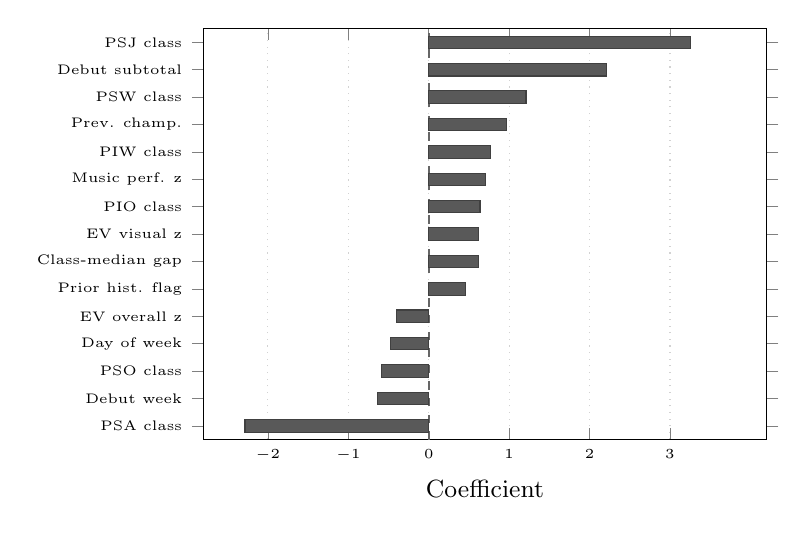
\begin{tikzpicture}
\begin{axis}[
  xbar,
  width=0.72\columnwidth,
  height=6.8cm,
  bar width=4.5pt,
  xlabel={Coefficient},
  xlabel style={font=\small},
  tick label style={font=\tiny},
  xmin=-2.8, xmax=4.2,
  xtick={-2,-1,0,1,2,3},
  ymin=-0.5, ymax=14.5,
  ytick={0,1,2,3,4,5,6,7,8,9,10,11,12,13,14},
  yticklabels={
    PSA class,
    Debut week,
    PSO class,
    Day of week,
    EV overall z,
    Prior hist. flag,
    Class-median gap,
    EV visual z,
    PIO class,
    Music perf. z,
    PIW class,
    Prev. champ.,
    PSW class,
    Debut subtotal,
    PSJ class,
  },
  xmajorgrids=true,
  grid style={dotted, gray!35},
  extra x ticks={0},
  extra x tick labels={},
  extra x tick style={
    grid=major,
    grid style={black!60, dashed, line width=0.7pt},
    tick style={draw=none},
  },
]
\addplot[
  fill=black!65,
  draw=black!75,
] coordinates {
  (-2.2845,0)
  (-0.6380,1)
  (-0.5830,2)
  (-0.4727,3)
  (-0.4000,4)
  (0.4579,5)
  (0.6232,6)
  (0.6234,7)
  (0.6378,8)
  (0.7016,9)
  (0.7704,10)
  (0.9724,11)
  (1.2092,12)
  (2.2151,13)
  (3.2527,14)
};
\end{axis}
\end{tikzpicture}
\caption{Top 15 Ridge regression coefficients by absolute magnitude. Class coefficients are relative to PIA, the omitted reference category; reference class choice affects coefficient scale but not model predictions. Positive values indicate higher predicted championship subtotal; negative indicate lower. Debut subtotal and class membership dominate; prior championship subtotal adds incremental signal.}
\Description{Horizontal bar chart of the 15 largest standardized Ridge coefficients. Debut subtotal and several class indicators have the largest magnitudes.}
\label{fig:ridge-coefficients}
\end{figure}
